\documentclass[12 pt, a4paper]{article}
\usepackage[english]{babel}  								% For norsk oppsett
\usepackage[utf8]{inputenc}
\usepackage{amsmath}
\usepackage{amssymb}
\usepackage{graphicx}
\usepackage{tabularx}
\usepackage{subcaption}
\usepackage{hyperref}
\usepackage{fancyhdr}
\usepackage{enumerate}
\usepackage{float}
\usepackage{tikz}
\usepackage{fancyhdr}
\usepackage{lastpage}
\usepackage{circuitikz}
\usepackage{physics}
\usepackage[includeheadfoot, margin =0.5 in]{geometry}
\usepackage[FYS, OnlyFrontpage]{mnfrontpage} 			%SKIFT HER!!!
\usepackage[version=3]{mhchem}
\usepackage{biblatex}%,style=numeric-comp
%\usepackage{cite}
\usepackage{siunitx}
\usepackage{todonotes}
\usepackage{xcolor}
\usepackage{listings}
%%%%
\usepackage[bottom]{footmisc}
\renewcommand\footnoterule{\rule{\linewidth}{0.5pt}}
%\renewcommand[\footnoterule]{%
%	\kern -3pt
%	\hrule width \textwidth height 1pt
%	\kern 2pt
%}
%%%%
\lstset{basicstyle=\ttfamily,
  showstringspaces=false,
  commentstyle=\color{red},
  keywordstyle=\color{blue}
}
%\usepackage{showframe}  %Dette viser hvordan strukturen på sidene er

\setlength{\parindent}{0cm}

\author{
\href{https://scontent-frx5-1.xx.fbcdn.net/v/t31.0-8/12671762_10153383742266712_8474119290530634136_o.jpg?_nc_cat=101&oh=b9e610135e542e9665afa60c4ce37e77&oe=5C2C51F3}{Erik Skaar}\\
\href{https://scontent-arn2-1.xx.fbcdn.net/v/t1.0-9/37684668_10215236585082209_7481237283308306432_o.jpg?_nc_cat=107&oh=40a14b829370efbefb24835cb1cc58e3&oe=5C25967D}{Sondre Torp}\\
\href{https://scontent-arn2-1.xx.fbcdn.net/v/t1.0-9/14068064_10153996427056633_4906324953345045605_n.jpg?_nc_cat=111&oh=73976955adace15b21b1c44f36cdca1d&oe=5C25BAA0}{Mikael Kiste}
}



\bibliography{kilder.bib}

\font\myfont=cmr12 at 35pt
\title{\textbf{{\myfont Monte Carlo Modeling of Transactions}}}
\begin{document}
\mnfrontpage


\pagestyle{fancy}
\fancyhf{}
\rhead{FYS-STK4155}
\lhead{\href{https://github.com/erikfsk/Project-5}{Erik Skaar}}
\fancyfoot[CE,LO]{\leftmark}
\fancyfoot[LE,RO]{Page \number\value{page} of \pageref{LastPage}}

\renewcommand{\headrulewidth}{2pt}
\renewcommand{\footrulewidth}{1pt}

\tableofcontents



\pagebreak
\pagebreak
\section*{Abstract}%1
This report is based on a project assignment in the subject FYS-STK4155 at UiO.\cite{project1}
In this report the following regression methods were implemented; OLS, ridge and Lasso.
To understand how well our methods worked, we tested it against Scikit's solutions,
checked time dependance for different order of fitting and checked how noise affected the
resulting polynomial. Then our implementation, OLS, Ridge and Lasso, were used on the Franke function.
MSE,R2 score and VAR was calculated for all of the methods and how k-fold cross validation
affected to resulting polynomial is shown. After this had been done on the Franke function,
we repeated the proccedure for terrain data in Norway. The resulting polynomial were a good
approximation for general features for the data, but fell short to describe the details.

\cite{compphys}


\section{Introduction}
\input{intro/intro}


\section{Theory}\label{sec:theory}
\subsection{Standard}


\begin{align*}
    \beta = \left(
    \textbf{X}^T\textbf{X}
    \right)^{-1}
    \textbf{X}^T\textbf{y}
\end{align*}

\subsection{Ridge}

\begin{align*}
    \beta = \left(
    \textbf{X}^T\textbf{X}
     + \lambda \textbf{I}
     \right)^{-1}
    \textbf{X}^T\textbf{y}
\end{align*}

\subsection{Lasso}

\begin{align*}
    \beta = \text{argmin}_{\beta}
    \left\{
    \sum^N_{i=1}
    \left(
    y_i - \beta_0 -
    \sum_{j=1}^p x_{ij}\beta_j
    \right)^2
    + \lambda
    \sum^p_{j=1}|\beta_j|^q
    \right\}
\end{align*}


\subsection{k-fold and bootstrap}




\section{Method}

\pagebreak
\section{Implementation}

The three different algorithms discussed in section xxx was implemented in
\href{https://github.com/erikfsk/fysstk4155-project-1/blob/master/project/project-e.py}{\color{blue}{our script}}.
It is a few different versions, but the \"e\" version contains all you need.
All the scripts discussed in this report can be found at
\href{https://github.com/erikfsk/fysstk4155-project-1/}{\color{blue}{our github}}.
\\
\\
The program was tested on the Frank-function, see equation \ref{eq:Franke}.
With an known solution we did a k-fold test and an degree and $\lambda$/$\alpha$ test.
Both tested was done with the script descriped earlier.
The tables below shows the different results.

\begin{align}
f(x,y) &=
\frac{3}{4} e^{\left(-\frac{(9x-2)^2}{4} - \frac{(9y-2)^2}{4}\right)}
+\frac{3}{4} e^{\left(-\frac{(9x+1)^2}{49}- \frac{(9y+1)}{10}\right)}
+\frac{1}{2} e^{\left(-\frac{(9x-7)^2}{4} - \frac{(9y-3)^2}{4}\right)}
 -\frac{1}{5} e^{\left(-(9x-4)^2 - (9y-7)^2\right)}
\label{eq:Franke}
\end{align}

\subsection{Scikit vs. manually implementation}

\begin{figure}[H]
    \centering
    \begin{subfigure}{0.5\textwidth}
        \centering
        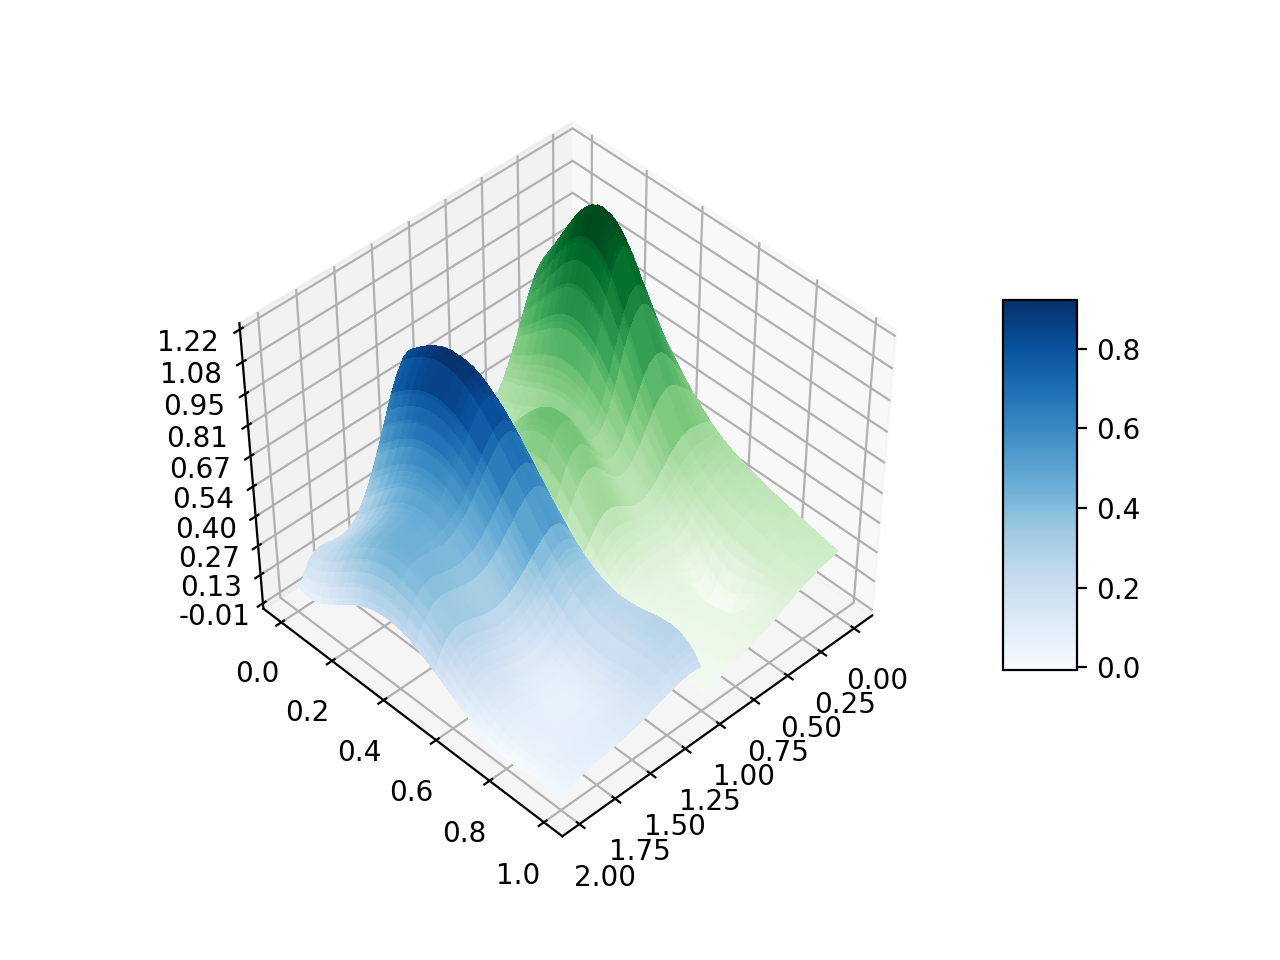
\includegraphics[width=\linewidth]{method/bilder/actual}
        \caption{}
    \end{subfigure}%
    ~
    \begin{subfigure}{0.5\textwidth}
        \centering
        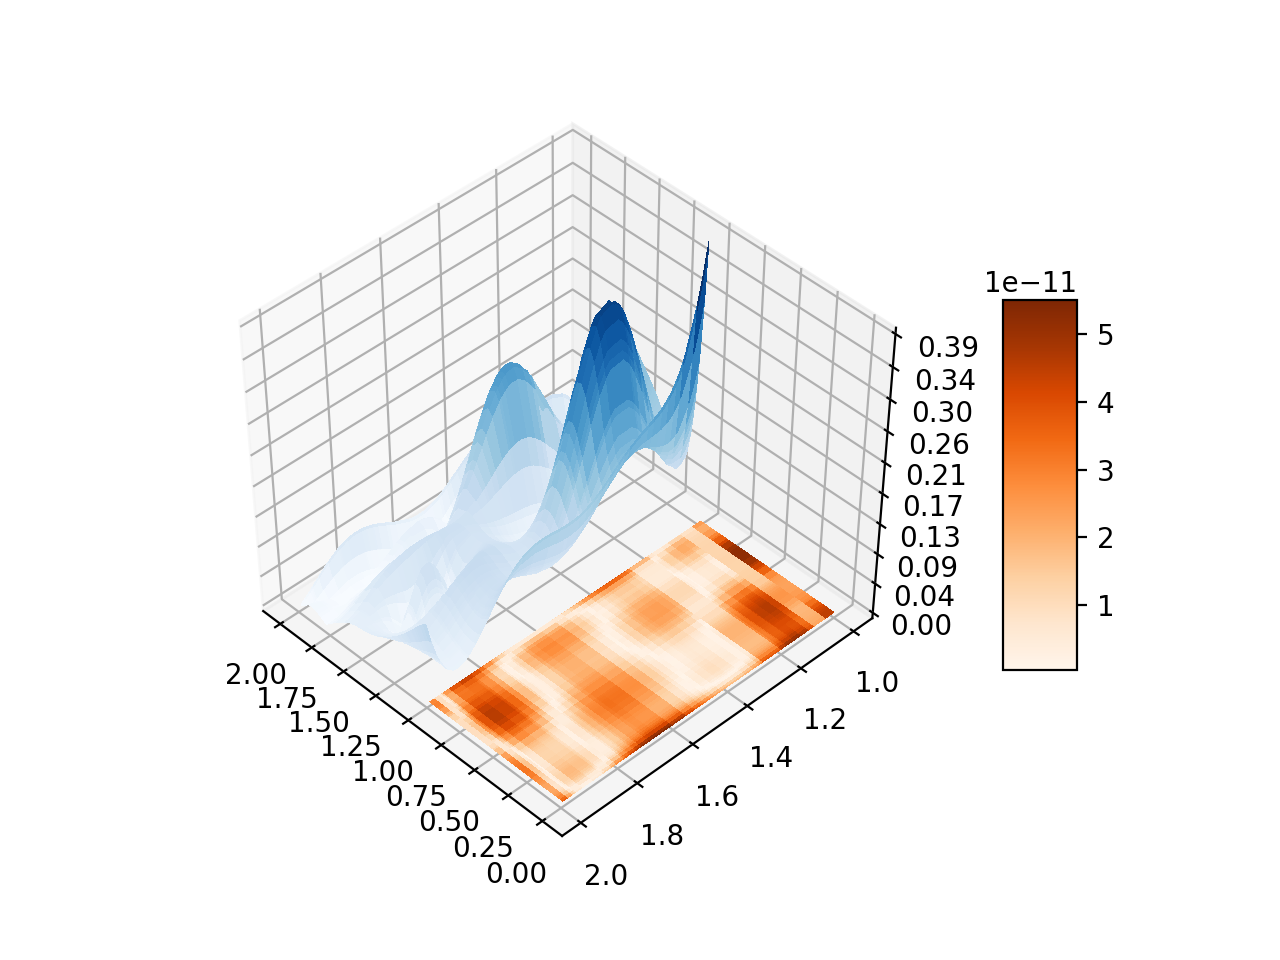
\includegraphics[width=\linewidth]{method/bilder/error}
        \caption{}
    \end{subfigure}
    \caption{a)... b)...}
    \label{fig:test}
\end{figure}

\subsection{Time evolution}

\begin{center}
\label{tab:time-test}
\captionof{table}{This tables shows how the MSE evoles for different degrees.
Scikit OLS is to confirm that our implementation is not retarded.
For lasso and ridge the $\lambda$/$\alpha$ was set to 1e-5.
Also, if we go beyond fifth order the OLS solutions starts to crumble.}
\begin{tabularx}{\textwidth}{l X c X c X c X c X c}
    \hline
    \hline
        degree $\downarrow$ && method $\rightarrow$ && OLS && SCIKIT && RIDGE && SCIKIT LASSO\\
    \hline
        $2  $               && &&   0.01517s &&	0.25830s	 &&	0.00516s      && 0.00543s		\\
        $2_{relative}$   	&& &&   1.00   	 &&	1.00 	     &&	1.00          &&	1.00	\\
        $3_{relative}$   	&& &&   2.42   	 &&	1.58	     &&	2.45          &&	2.38	\\
        $4_{relative}$   	&& &&   3.63   	 &&	2.45	     &&	5.11          &&	4.88	\\
        $5_{relative}$   	&& &&   4.98   	 &&	3.61	     &&	8.77          &&	8.31	\\
    \hline
\end{tabularx}
\end{center}

\subsection{Noise - MSE \& R2 evolution}

\begin{center}
\label{tab:noise-test-MSE}
\captionof{table}{This tables shows how the MSE evoles for different degrees.
Scikit OLS is to confirm that our implementation is not retarded.
For lasso and ridge the $\lambda$/$\alpha$ was set to 1e-5.
Also, if we go beyond fifth order the OLS solutions starts to crumble.}
\begin{tabularx}{\textwidth}{l X c X c X c X c X c}
    \hline
    \hline
        Noise level $\downarrow$ && method $\rightarrow$ && OLS && SCIKIT && RIDGE && SCIKIT LASSO\\
    \hline
        $0  $               && &&   0.00127     &&	0.00127	  &&	0.00514      && 0.00127		\\
        $0_{relative}$   	&& &&   1.00   	    &&	1.00 	  &&	1.00         &&	1.00	\\
        $0.01_{relative}$   && &&   1.03   	    &&	1.03	  &&	1.00         &&	1.03	\\
        $0.2_{relative}$   	&& &&   12.84   	&&	12.84	  &&	3.68         &&	12.84	\\
        $0.5_{relative}$   	&& &&   42.04   	&&	42.04	  &&	10.84        &&	42.04	\\
    \hline
\end{tabularx}
\end{center}

\begin{center}
\label{tab:noise-test-R2}
\captionof{table}{This tables shows how the MSE evoles for different degrees.
Scikit OLS is to confirm that our implementation is not retarded.
For lasso and ridge the $\lambda$/$\alpha$ was set to 1e-5.
Also, if we go beyond fifth order the OLS solutions starts to crumble.}
\begin{tabularx}{\textwidth}{l X c X c X c X c X c}
    \hline
    \hline
        Noise level $\downarrow$ && method $\rightarrow$ && OLS && SCIKIT && RIDGE && SCIKIT LASSO\\
    \hline
        $0$   	    && &&   0.98  	&&	0.98	  &&   0.91         &&	0.98    \\
        $0.01$      && &&   0.98  	&&	0.98      &&   0.91         &&	0.98    \\
        $0.2$   	&& &&   0.68   	&&	0.68	  &&   0.62         &&	0.68	\\
        $0.5$   	&& &&   0.28   	&&	0.28	  &&   0.25        &&	0.28	\\
    \hline
\end{tabularx}
\end{center}




\section{Result \& Discussion}

\subsection{Ordinary least square, Ridge, and Lasso regression with resampling on the Franke function}

In this subsection we will present our results from Ordinary least square, Ridge and Lasso regression, up to the fifth order, with a resampling technic, k-fold, on the Franke function. The Mean square error, (MSE), $R^2$ score and the confidence intervall from the calculations are also presented, these values were found by taking the average values over a 100 different executions, with a noise level $= 0.1$ and a $\lambda = 0.00001$.


\subsubsection{Ordinary least square}
Here we present our results on the OLS regression with up to a fifth order polynomial fit on Franke function, notice that in the plot we use a fifth order polynomial, the $R^2$ score and MSE according to order of the polynomial used for fitting of the data. And lastly a table containing the $\beta$ values, the variance, and the confidence intervall according to the different polynomials.

%The confidence intervall of $\beta$ through variance. The mean squared error(MSE) and the $R^2$ score function. 
%Presenting the resampling of the data, where the data have been splitt into training and test data. 
%Bias?


\begin{figure}[H]
\centering
      \begin{subfigure}{0.45\textwidth}
       	\centering
       	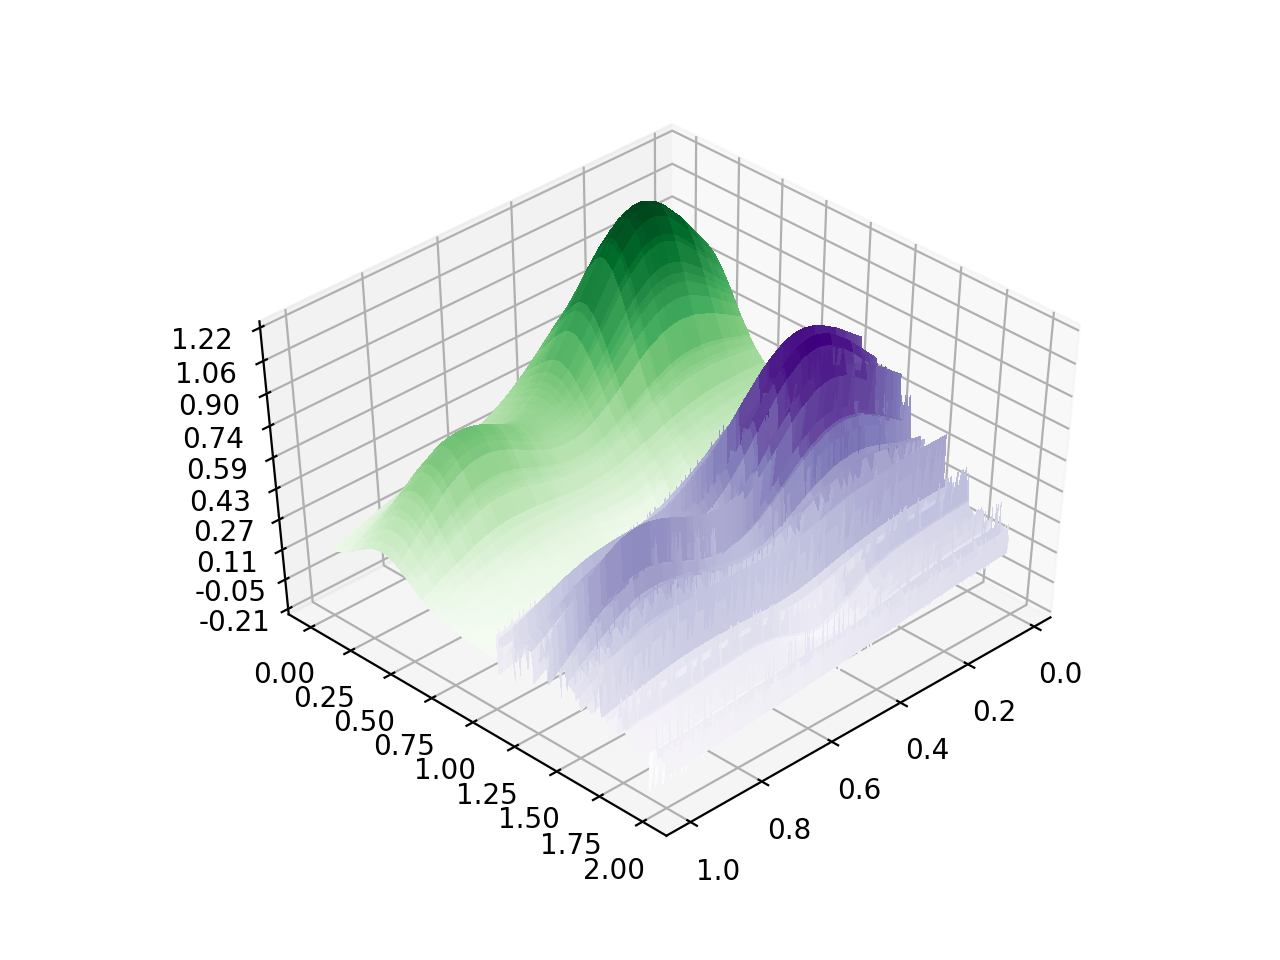
\includegraphics[width=\linewidth]{result/bilder/Franke_noise.png}
        	\caption{}
     \end{subfigure}
     ~
     \begin{subfigure}{0.45\textwidth}
       	\centering
       	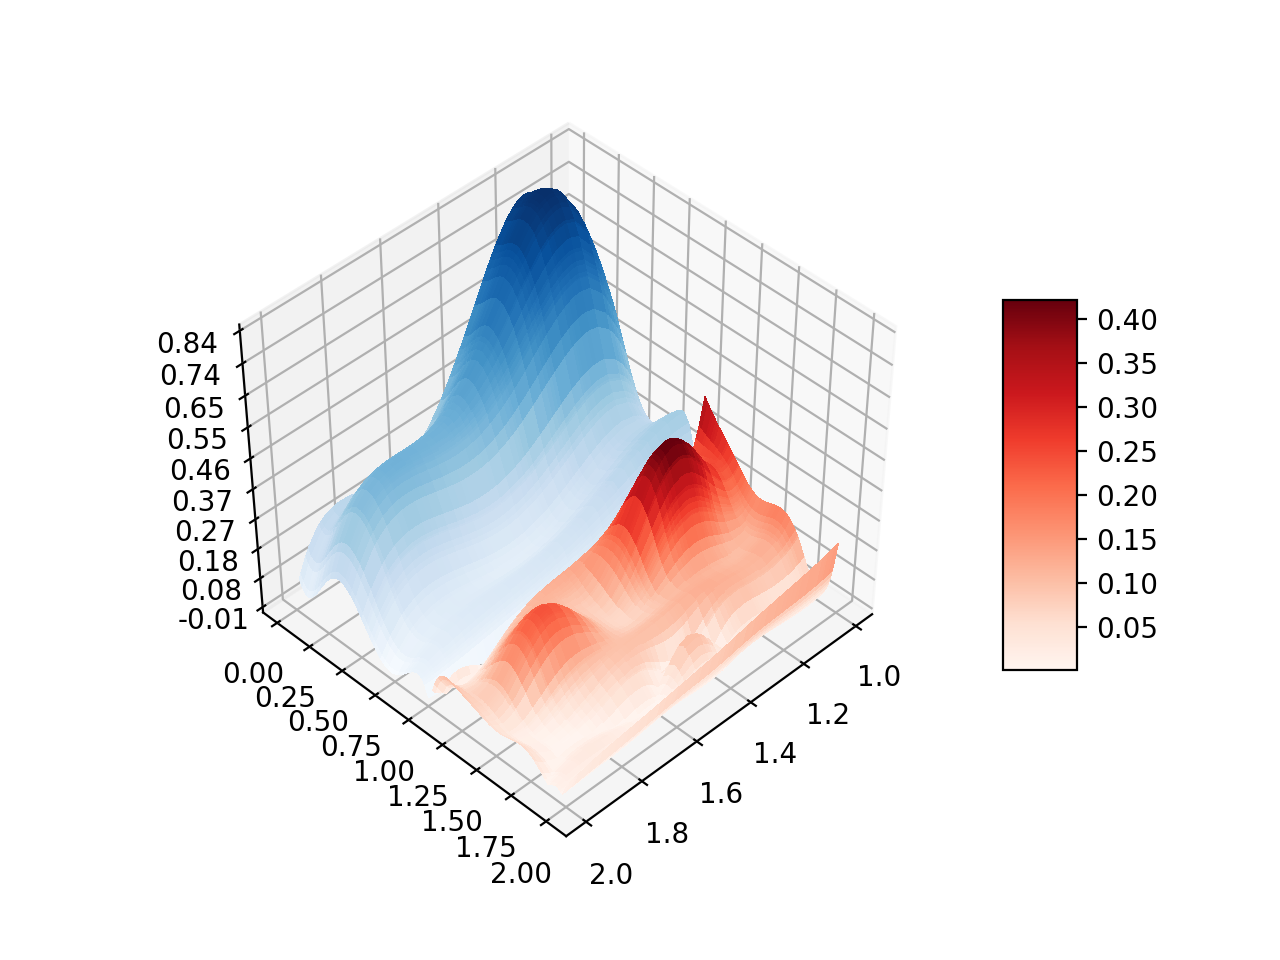
\includegraphics[width=\linewidth]{result/bilder/OLS_bar.png}
        	\caption{}
    	\end{subfigure}
 	\caption{a) \color{green}Franke function \color{black}, and the \color{purple}Frank function with noise plottet\color{black}. b) Our \color{blue}fifth order approximation of the Franke function\color{black}. On the right we have the \color{red}residuals\color{black}, i.e. the error compared to the real function, and its relative size indicated by the red colour gradient.}
	\label{fig:OLS_Frank}
\end{figure}


 \begin{center}
 \label{tab:OLS_Degree_R2_MSE}
 \captionof{table}{MSE and $R^2$ score for OLS by degree. These values are created by taking the average values over 100 different executions, with a noise level $= 0.1$ and a $\lambda = 0.00001$ }
 \begin{tabularx}{\textwidth}{c X c X c  }
     \hline
     \hline
         Degree && R2 && MSE \\
         \hline
2      && 0.71 && 0.01353 \\ 
3      && 0.81 && 0.00916 \\ 
4      && 0.86 && 0.00712 \\ 
5      && 0.88 && 0.00585 \\ \hline
 \end{tabularx}
 \end{center}
 
 \pagebreak
 \begin{center}
 \label{tab:OLS_lambda_R2_MSE}
 \captionof{table}{ MSE and $R^2$ score for OLS by $\lambda$, with a fifth order polynomial. These values are created by taking the average values over $100$ different executions, with a noise level $= 0.1$}
 \begin{tabularx}{\textwidth}{c X c X c  }
     \hline
     \hline
         $\lambda$ && R2 && MSE \\
         \hline
 0.0000001  && 0.87497  && 0.00587 \\
0.0000100  && 0.87517  && 0.00605 \\
0.0010000  && 0.87723  && 0.00592 \\
0.1000000  && 0.87242 && 0.00608 \\
1.0000000  && 0.87708 && 0.00613 \\
2.0000000  && 0.87833 && 0.00586 \\
5.0000000  && 0.87572 && 0.00601 \\
10.0000000 && 0.87528 && 0.00591\\ \hline
 \end{tabularx}
 \end{center}

  \begin{center}
 \label{tab:Confidenceintervall_OLS}
 \captionof{table}{$\beta$, Var and Confidence intervall for OLS by degree of $x$ and $y$. }
 \begin{tabularx}{\textwidth}{c X l X l X l }
     \hline
     \hline
     $x^iy^j$ && $\beta$ && VAR && Confidence intervall \\
     \hline
$x^0y^0$     && 0.259   && 0.001   &&  [0.227, 0.291]     \\ 
$x^0y^1$     && 4.117   && 0.108   &&  [3.788, 4.446]     \\ 
$x^0y^2$     && -18.065 && 2.943   &&  [-19.781, -16.349] \\ 
$x^0y^3$     && 29.764  && 15.934  &&  [25.772, 33.756]   \\ 
$x^0y^4$     && -22.199 && 17.571  &&  [-26.391, -18.007] \\ 
$x^0y^5$     && 6.361   && 2.637   &&  [4.737, 7.985]     \\ 
$x^1y^0$     && 5.277   && 0.074   &&  [5.005, 5.549]     \\ 
$x^1y^1$     && -9.751  && 1.234   &&  [-10.862, -8.64]   \\ 
$x^1y^2$     && 13.591  && 6.186   &&  [11.104, 16.078]   \\ 
$x^1y^3$     && -21.609 && 7.858   &&  [-24.412, -18.806] \\ 
$x^1y^4$     && 12.635  && 1.628   &&  [11.359, 13.911]   \\ 
$x^2y^0$     && -22.726 && 1.825   &&  [-24.077, -21.375] \\ 
$x^2y^1$     && 28.964  && 5.900   &&  [26.535, 31.393]   \\ 
$x^2y^2$     && -1.849  && 6.149   &&  [-4.329, 0.631]    \\ 
$x^2y^3$     && -5.401  && 1.364   &&  [-6.569, -4.233]   \\ 
$x^3y^0$     && 30.056  && 10.123  &&  [26.874, 33.238]   \\ 
$x^3y^1$     && -36.035 && 7.072   &&  [-38.694, -33.376] \\ 
$x^3y^2$     && 6.742   && 1.441   &&  [5.542, 7.942]     \\ 
$x^4y^0$     && -11.919 && 12.008  &&  [-15.384, -8.454]  \\ 
$x^4y^1$     && 12.813  && 1.444   &&  [11.611, 14.015]   \\ 
$x^5y^0$     && -0.909  && 1.951   &&  [-2.306, 0.488]    \\ 

     \hline
 \end{tabularx}
 \end{center}

 
\subsubsection{Ridge regression}
The results from the Ridge calculations are here presented in the same manner as for Ordinary least square. Again finding the MSE, $R^2$ score, according to polynomial degree, and testing for different $\lambda$. Finding the $\beta$ values, VAR, and the Confidence intervall. We see here that the $R^2$ score is unstable for higher values of $\lambda$.
 
 \pagebreak
 \begin{center}
 \label{tab:Ridge_Degree_R2_MSE}
 \captionof{table}{MSE and $R^2$ score for Ridge by degree. These values are created by taking the average values over 100 different executions, with a noise level $= 0.1$ and a $\lambda = 0.00001$.}
 \begin{tabularx}{\textwidth}{c X c X c  }
     \hline
     \hline
         Degree && R2 && MSE \\
         \hline
2      && 0.71 && 0.01353 \\ 
3      && 0.80 && 0.00968 \\ 
4      && 0.81 && 0.00928 \\ 
5      && 0.81 && 0.00902 \\ \hline
 \end{tabularx}
 \end{center}
 
 
\begin{center}
 \label{tab:OLS_lambda_R2_MSE}
 \captionof{table}{ MSE and $R^2$ score for Ridge $\lambda$. These values are created by taking the average values over $100$ different executions, with a noise level $= 0.1$.}
 \begin{tabularx}{\textwidth}{c X c X c  }
     \hline
     \hline
         $\lambda$ && R2 && MSE \\
         \hline
 0.0000001  && 0.81150  && 0.00894 \\
0.0000100  && 0.80979  && 0.00932 \\
0.0010000  && 0.74059  && 0.01237 \\
0.1000000  && -0.20901 && 0.05933 \\
1.0000000  && -1.85170 && 0.13474 \\
2.0000000  && -1.83823 && 0.14025 \\
5.0000000  && -1.79681 && 0.13813 \\
10.0000000 && -1.81950 && 0.13576\\ \hline
 \end{tabularx}
 \end{center}


  \begin{center}
 \label{tab:Confidenceintervall_Ridge}
 \captionof{table}{$\beta$, Var and Confidence intervall for Ridge by degree of $x$ and $y$. }
 \begin{tabularx}{\textwidth}{c X l X l X l }
     \hline
     \hline
     $x^iy^j$ && value && variance && Confidence intervall \\
     \hline
$x^0y^0$     && 0.384    && 0.001   && [0.352, 0.416]     \\
$x^0y^1$     && 1.770    && 0.077   && [1.493, 2.047]     \\
$x^0y^2$     && -0.294   && 1.953   && [-1.691, 1.103]    \\
$x^0y^3$     && -22.690  && 10.474  && [-25.926, -19.454] \\
$x^0y^4$     && 41.542   && 12.033  && [38.073, 45.011]   \\
$x^0y^5$     && -20.675  && 1.949   && [-22.071, -19.279] \\
$x^1y^0$     && 5.348    && 0.068   && [5.087, 5.609]     \\
$x^1y^1$     && -11.544  && 1.040   && [-12.564, -10.524] \\
$x^1y^2$     && 18.567   && 4.891   && [16.355, 20.779]   \\
$x^1y^3$     && -27.573  && 6.071   && [-30.037, -25.109] \\
$x^1y^4$     && 14.943   && 1.295   && [13.805, 16.081]   \\
$x^2y^0$     && -21.987  && 1.712   && [-23.295, -20.679] \\
$x^2y^1$     && 32.153   && 5.221   && [29.868, 34.438]   \\
$x^2y^2$     && -5.093   && 5.179   && [-7.369, -2.817]   \\
$x^2y^3$     && -3.142   && 1.161   && [-4.219, -2.065]   \\
$x^3y^0$     && 25.775   && 9.426   && [22.705, 28.845]   \\
$x^3y^1$     && -39.259  && 6.976   && [-41.9, -36.618]   \\
$x^3y^2$     && 6.673    && 1.214   && [5.571, 7.775]     \\
$x^4y^0$     && -4.833   && 11.244  && [-8.186, -1.48]    \\
$x^4y^1$     && 14.552   && 1.590   && [13.291, 15.813]   \\
$x^5y^0$     && -4.681   && 1.908   && [-6.062, -3.3]    \\ 
    \hline
 \end{tabularx}
 \end{center}      

 

\subsubsection{Lasso regression}
The results from the Lasso regression, again presenting the MSE, $R^2$, $\beta$, VAR, and Confidence interval.


 \begin{center}
 \label{tab:Lasso_Degree_R2_MSE}
 \captionof{table}{MSE and $R^2$ score for Lasso by degree. These values are created by taking the average values over 100 different executions, with a noise level $= 0.1$ and a $\lambda = 0.00001$}
 \begin{tabularx}{\textwidth}{c X c X c  }
     \hline
     \hline
         Degree && R2 && MSE \\
         \hline
2      && 0.71 && 0.01353 \\ 
3      && 0.81 && 0.00916 \\ 
4      && 0.86 && 0.00712 \\ 
5      && 0.88 && 0.00585 \\ \hline
 \end{tabularx}
 \end{center}
 
 
 \begin{center}
 \label{tab:Degree_R2_MSE}
 \captionof{table}{MSE and $R^2$ score for Lasso on Franke function by $\lambda$. These values are created by taking the average values over 100 different executions, with a noise level $= 0.1$}
 \begin{tabularx}{\textwidth}{c X c X c  }
     \hline
     \hline
$\lambda$    &&R2     &&MSE     \\
         \hline
0.0000001 &&0.87497&&0.00587 \\
0.0000100 &&0.87517&&0.00605 \\
0.0010000 &&0.87723&&0.00592 \\
0.1000000 &&0.87242&&0.00608 \\
1.0000000 &&0.87708&&0.00613 \\
2.0000000 &&0.87833&&0.00586 \\
5.0000000 &&0.87572&&0.00601 \\
10.0000000 && 0.87528&&0.00591
 \end{tabularx}
 \end{center}
 
 \begin{center}
\label{tab:lasso-var-conf}
\captionof{table}{$\beta$, Var and Confidence intervall for Ridge by degree of $x$ and $y$. We have here cut the values for higher degrees because these were equal to zero.}
\begin{tabularx}{\textwidth}{c X c X c X l}
    \hline
    \hline
        $x^iy^j$ && $\beta$ && VAR && Confidens interval\\
    \hline
        $x^0y^0$ && 0.342129   && 0.000080   && [0.333197,0.351061] \\
        $x^0y^1$ && -0.437389  && 0.000347   && [-0.456013,-0.418765] \\
        $x^0y^2$ && -0.016612  && 0.000261   && [-0.032765,-0.000458] \\
        $x^0y^5$ && 0.000024   && 0.000000   && [-0.000140,0.000188] \\
        $x^1y^0$ && 0.558845   && 0.000299   && [0.541543,0.576146] \\
        $x^1y^1$ && -0.389778  && 0.000394   && [-0.409623,-0.369933] \\
        $x^3y^0$ && -0.000178  && 0.000001   && [-0.000933,0.000576] \\
        $x^4y^0$ && -0.120878  && 0.000436   && [-0.141758,-0.099998] \\
    \hline
\end{tabularx}
\end{center}


 
\subsection{Ordinary least square, Ridge, and Lasso regression with resampling, now on real data}

\begin{figure}[H]
		\centering
		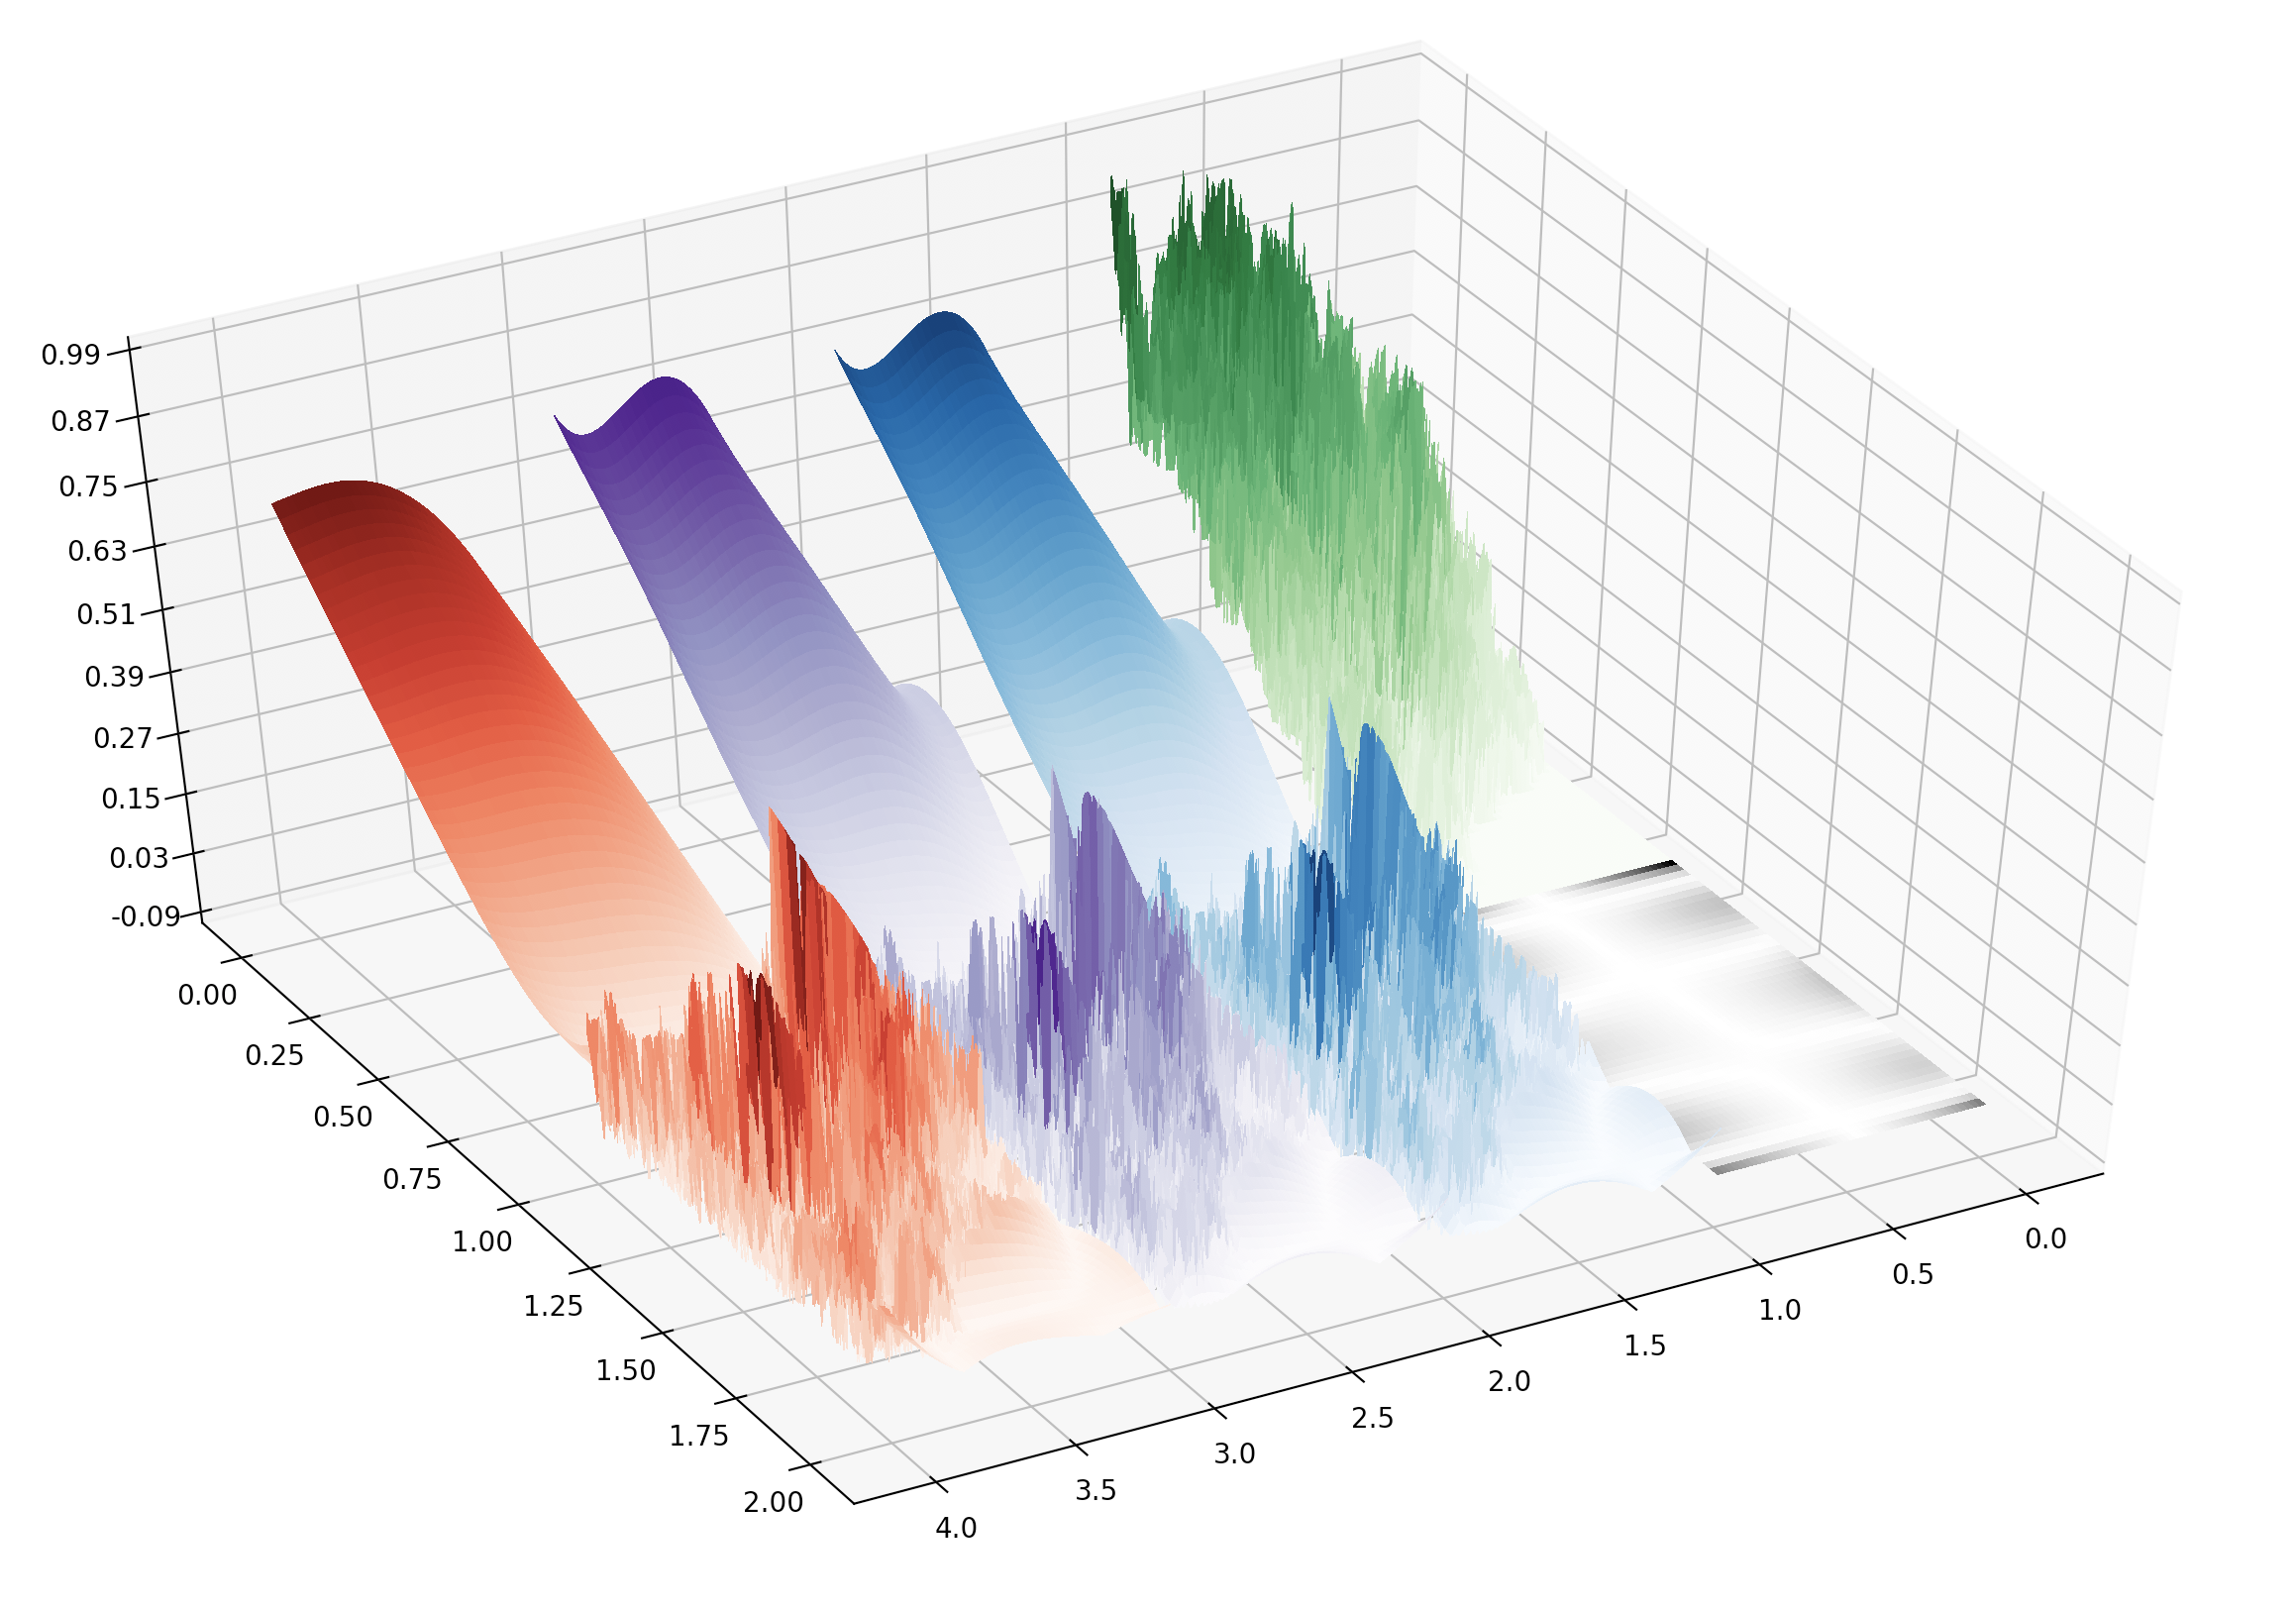
\includegraphics[width=1.1\linewidth]{result/bilder/all_real.png}
		\caption{From left to right: The \color{red}OLS \color{black} regression, \color{purple}{} Ridge \color{black} regression, \color{blue} Lasso \color{black} regression, and the \color{green}Real data \color{black} that we tried to approximate, with their residuals.}
		\label{fig:RealData}
\end{figure}


 \begin{center}
 \label{tab:Realdata_OLS_lambda_R2_MSE}
 \captionof{table}{OLS regression on Real data. }
 \begin{tabularx}{\textwidth}{c X c X c  }
     \hline
     \hline
$\lambda$    &&R2     &&MSE     \\
         \hline
0.0000001 && 0.823088 && 0.010720 \\
0.0000100 && 0.823088 && 0.010720 \\
0.0010000 && 0.823088 && 0.010720 \\
0.1000000 && 0.823088 && 0.010720 \\
 \end{tabularx}
 \end{center}
 
\pagebreak
 
 \begin{center}
 \label{tab:Realdata_Lasso_lambda_R2_MSE}
 \captionof{table}{Lasso on realdata. We saw that $R^2$ got out of hand with a $\lambda = 0.1$ and higher, and decided not to include those numbers. }
 \begin{tabularx}{\textwidth}{c X c X c  }
     \hline
     \hline
$\lambda$    &&R2     &&MSE     \\
         \hline
0.0000001 && 0.797486 && 0.012272 \\
0.0000100 && 0.797470 && 0.012273 \\
0.0010000 && 0.753280 && 0.014950 \\
0.1000000 && -0.165026 && 0.070596 \\
 \end{tabularx}
 \end{center}

 \begin{center}
 \label{tab:Realdata_Ridge_lambda_R2_MSE}
 \captionof{table}{Ridge on realdata. MSE and $R^2$ score for Ridge on the real data by $\lambda$. }
 \begin{tabularx}{\textwidth}{c X c X c  }
     \hline
     \hline
$\lambda$    &&R2     &&MSE     \\
         \hline
0.0000001 && 0.823088 && 0.010720 \\
0.0000100 && 0.823088 && 0.010720 \\
0.0010000 && 0.823027 && 0.010724 \\
0.1000000 && 0.818116 && 0.011022 \\
 \end{tabularx}
 \end{center}





%Presenter en kristisk vurdering og diskuter applikasjonsmulighetene(applicability) av disse regresjonsmetodene til typen data som blir presentert her. DISKUSJONSDEL





%\pagebreak
%\section{Discussion}
%\input{discussion/discussion}


\section{Conclusion}
We have seen how the different models behave. The time was almosst irrelevant for choosing
OLS, Ridge or Lasso. The k-folding technique reduced the time and also preserved the R2 score and MSE.
The Lasso might not be the best fit to the real data, but it has the simplest model.
It has 8 coefficient, compared to 21 for Ridge and OLS. If the module was meant to predict
new values, Lasso would save you 13 FLOPs per prediction, while only droping slightly in R2
score and MSE accuracy. A pretty good deal if many predictions are needed with the model. An other conclusion
that might be as interesting is that we should keep using the Scikit package. Our code...
Well, it did not perform as well as we would have liked.
\\
\\
\\
\\
\\
\\
\\
\\
\\
\\
\\
\\
\\
\\
\\
\\
\\
\\



\printbibliography

\section{Appendix}\label{sec:appendix}
\input{appendix/appendix}





% \begin{figure}[H]
%     \centering
%     \begin{subfigure}{0.5\textwidth}
%         \centering
%         \includegraphics[width=\linewidth]{result/bilder/...}
%         \caption{}
%     \end{subfigure}%
%     ~
%     \begin{subfigure}{0.5\textwidth}
%         \centering
%         \includegraphics[width=\linewidth]{result/bilder/...}
%         \caption{}
%     \end{subfigure}
%     \caption{a)... b)...}
%     \label{fig:test}
% \end{figure}




% \begin{center}
% \label{tab:test}
% \captionof{table}{}
% \begin{tabularx}{\textwidth}{c X c X c X c }
%     \hline
%     \hline
%         $L_i$ && $T_C(L_i)$ && $T_C(\infty)$ with $\overline{a}$ \\
%     \hline
%         60      &&  2.30  && 2.2999\\
%         100     &&  2.29  && 2.2899\\
%         140     &&  2.28  && 2.2799\\
%         200     &&  2.27  && 2.2699\\
%     \hline
% \end{tabularx}
% \end{center}









%\begin{align*}
%&n \qquad &2^n - (-1)^n\\
%&n+1 \qquad &2^{n+1} - (-1)^{n+1} \\
%& &= 2(2^{n}) - (-1)^{n+1}\\
%& &= 2(2^{n} + (-1)^n  + (-1)^{n+1}) - (-1)^{n+1}\\
%& &= 2(2^{n} + (-1)^n  - (-1)^{n}) - (-1)^{n+1}\\
%& &= 2(2^{n}- (-1)^{n}) + 2(-1)^n  + (-1)^{n}\\
%& &= 2(2^{n}- (-1)^{n}) + 3(-1)^n \\
%\end{align*}


%\begin{figure}[H]
%		\centering
%		\includegraphics[width=0.7\linewidth]{ab.png}
%		\caption{Atomene er gule kuler, de elementære vektorene er blå og a vektorene er grønne.}
%		\label{fig:ab}
%\end{figure}

%\begin{tabular}{|c|c|c|c|c|c|c|}
%	\hline
%	n & General & Specific & LU & fastest & slowest & $\frac{slowest}{fastest}$\\
%	\hline
%	10 & 6.5e-05 & 5e-06 & 4e-05 & Specific & General & 13.0\\
%	\hline
%	100 & 7.5e-05 & 8e-06 & 0.0023 & Specific & LU & 287.5\\
%	\hline
%	1000 & 0.00014 & 4e-05 & 0.26 & Specific & LU & 6500\\
%	\hline
%	10000 & 0.0007 & 0.0005 & 142.5 & Specific & LU & 285000 \\
%	\hline
%\end{tabular}


\end{document}
